\cleardoublepage

\chapter{Servidor de datos}
\label{makereference3}

\section{Introducción}
\label{makereference3.1}
La información recogida por el nodo es almacenada en un servidor central (al que llamamos ``servidor de datos''). Este se encarga de recibir la información proporcionada por uno o varios clientes (el nodo en nuestro caso), almacenarla y distribuirla a quien la requiera.

La comunicación se realiza sobre el protocolo MQTT muy utilizado para la comunicación máquina a máquina. Como implementación de este protocolo utilizamos el servidor \href{https://mosquitto.org/}{mosquitto}.

\section{MQTT}
\label{makereference3.2}
\textbf{MQTT} o lo que es lo mismo \textit{Message Queue Telemetry Transpor}t es un protocolo para la comunicación \textbf{machine-to-machine} de mensajería muy simple y ligero, orientado a conexión por \textbf{TCP/IP}. Esta diseñado principalmente para dispositivos con poco ancho de banda y con latencia baja.

MQTT es un servicio de publicación/suscripción TCP/IP sencillo y muy ligero. Se basa en el principio cliente/servidor y suscriptor/publicador.

El servidor, llamado broker, recopila los datos que los publicadores (``publishers'' en adelante) le transmiten. Determinados datos recopilados por el broker se enviarán a determinados publishers que previamente así se lo hayan solicitado al broker.

Los publishers envían los mensajes a un canal llamado topic. Los suscriptores (``subscribers'') pueden leer esos mensajes. Los topics (o canales de información) pueden estar distribuidos jerárquicamente de forma que se puedan seleccionar exactamente las informaciones que se desean.

La disposición jerárquica de estos ``topics'' está especialmente diseñada para facilitar la distribución de ``publishers'' y ``suscribers'' por grupos. De esta forma, si tuvieramos una instalación domótica podríamos distribuir los elementos a controlar en grupos jerárquicos.

Los mensajes enviados por los dispositivos comunicantes pueden ser de todo tipo pero no pueden superar los 256 Mb.

\subsection{Seguridad}
Los datos de IoT intercambiados pueden resultar muy críticos, por lo que es posible garantizar la seguridad de los intercambios en varios niveles:
\begin{itemize}
\item Transporte en SSL/TLS.
\item Autenticación mediante certificados SSL/TLS.
\item Autenticación mediante usuario y contraseña.
\end{itemize}

Este proyecto no utiliza ninguna de estas tres medidas de seguridad pero deberían implementarse en un futuro ya que el objetivo último de este proyecto sería para la ayuda a la toma de decisiones y no los datos no deberían poder verse afectados.

\subsection{QoS}
El protocolo MQTT define tres modos diferentes de asegurar la Calidad del Servicio (QoS, Quality of Service) que el publicador podrá definir según sus necesidades.

Hay tres niveles posibles:
\begin{itemize}
\item QoS nivel 0 (At Most Once) se entregará como mucho una vez por lo que el mensaje no tiene garantías de recepción (el broker no informa al publicador de que ha recibido el mensaje).

\item Qos nivel 1 (At Least Once) se entregará al menos una vez. El publicador lo transmitirá varias veces si es necesario, hasta que el broker le confirme que lo ha enviado a la red. Este es el nivel por defecto.

\item QoS nivel 2 (Exactly once) será obligatoriamente guardado por el emisor, que lo transmitirá siempre que el receptor no confirme su envío a la red.

En este proyecto no se define todavía un nivel de servicio pero sería interesante estudiar cuál de los tres es el más correcto para utilizar.
\end{itemize}

\begin{figure}[htb]
	\begin{center}
		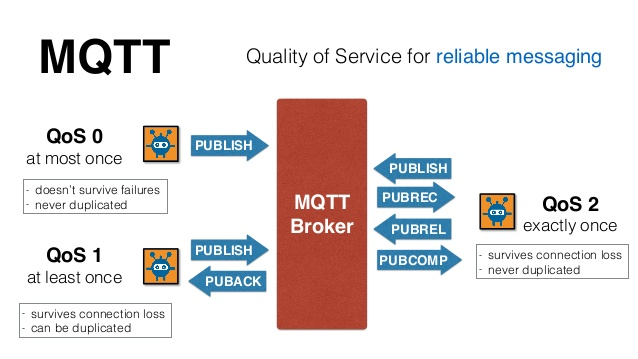
\includegraphics[height=8cm]{figures/mqtt-qos.jpg}
		\caption{Diagrama de los distintos niveles de calidad [Fuente: \href{https://image.slidesharecdn.com/0xwitjksqnqruoz4tnsi-signature-6a256d24caf5d1fcc6a3bf1d013dfe0e1fa99369a560d140998f50cbdbc6d127-poli-140828123252-phpapp02/95/mqtt-a-practical-protocol-for-the-internet-of-things-15-638.jpg?cb=1409229409}{SlideShare: MQTT - A practical protocol for the Internet of Thing}]}
	\end{center}

	\label{types}
\end{figure}

\subsection{Ventajas}
\begin{itemize}  
\item Utiliza un ancho de banda mínimo. Tiene una cabecera fija de 2 bytes más una cabecera variable. De este variable, durante la suscripción y conexión se utilizan 12 bytes. La mayoría de publicaciones utilizan 2 bytes de cabeceras variables.
\item Consume muy poca energía.
\item Permite una gran fiabilidad si es necesario por la definición de la QoS (Calidad de Servicio).
\item Requiere pocos recursos.
\end{itemize}

\subsection{Alternativas a MQTT}
Algunas de las alternativas que podemos encontrar a MQTT son las siguientes:

\begin{itemize}  
\item \href{https://www.lora-alliance.org/What-Is-LoRa/Technology}{LoRa} (Long Range) es una tecnología que ofrece un \textbf{largo alcance}, un \textbf{bajo consumo} de energía y una \textbf{transmisión segura} de datos. Entre sus ventajas cabe señalar que permite aplicaciones de seguimiento sin \textbf{GPS}, tiene un bajo coste y una alta capacidad, ideal para operadores de \textbf{redes públicas.}
\item \href{https://en.wikipedia.org/wiki/Constrained_Application_Protocol}{CoAP} (Constrained Application Protocol) es un protocolo que está diseñado para la transferencia de documentos entre \textbf{dispositivos restringidos.} Dentro de sus ventajas podemos destacar que está destinado para su uso en dispositivos de Internet con recursos limitados, está diseñado para \textbf{traducir fácilmente a HTTP.}
\item \href{https://www.amqp.org/}{AMQP} (Advanced Message Queuing Protocol) destaca por su orientación a la \textbf{mensajería de negocios.} Regula el comportamiento tanto del servidor como del cliente de la mensajería logrando que las implementaciones de diferentes proveedores sean \textbf{interoperables.} Esta es una de sus características más señaladas.
\end{itemize}
